\chapter{Pure Substances and Mixtures}\label{ch:g6:pure-substances-and-mixtures}

A bottle of mineral water lists on its label a dozen dissolved
substances, with their amounts in milligrams per litre. The water that
comes out of a laboratory's purifier lists none. Both are clear and
colourless, both quench thirst --- yet only one of them is what a
chemist calls pure. This chapter gives the word ``pure'' its exact
meaning, and shows how to tell a \omterm{def:g6:pure-substances-and-mixtures:pure-substance}{pure substance} from a \omterm{def:g6:pure-substances-and-mixtures:mixture}{mixture} without
tasting anything.

\begin{recall}
To \omterm{def:g2:mixing-and-dissolving:mix}{mix} is to put different things together; a solid that \omterm{def:g2:mixing-and-dissolving:dissolve}{dissolves} in
water leaves the liquid clear, and the clear liquid is a solution
(\cref{ch:g2:mixing-and-dissolving}). \omterm{def:g2:mixing-and-dissolving:mix}{Mixes} can be taken apart by
\omterm{def:g3:separating-mixtures:sieve}{sieving}, \omterm{def:g3:separating-mixtures:decant}{decanting}, \omterm{def:g3:separating-mixtures:filter}{filtering} and \omterm{def:g3:separating-mixtures:evaporate}{evaporating}
(\cref{ch:g3:separating-mixtures}). Every material has properties that
can be tested: hard or soft, transparent or not, floats or sinks
(\cref{ch:g1:materials-around-us}).
\end{recall}

\section{Chemical species and pure substances}

\begin{definition}[Chemical species]\label{def:g6:pure-substances-and-mixtures:species}
A \emph{chemical species}\index{chemical species} is one particular
kind of substance, with its own name and its own properties: water,
sugar, salt, oxygen, ethanol (the alcohol of wine), iron.
\end{definition}

\begin{definition}[Pure substance]\label{def:g6:pure-substances-and-mixtures:pure-substance}
A \emph{pure substance}\index{pure substance} is made of one single
\omterm{def:g6:pure-substances-and-mixtures:species}{chemical species} and nothing else: distilled water, a crystal of sugar,
a gold ring of pure gold.
\end{definition}

\begin{definition}[Mixture]\label{def:g6:pure-substances-and-mixtures:mixture}
A \emph{mixture}\index{mixture} contains several \omterm{def:g6:pure-substances-and-mixtures:species}{chemical species}. \omterm{def:g4:air-a-mixture-of-gases:air}{Air},
sea water, mineral water, milk, granite and orange juice are mixtures.
\end{definition}

\begin{remark}[Pure in everyday language]\label{rem:g6:pure-substances-and-mixtures:everyday}
A carton of ``pure orange juice'' means that nothing has been added to
the juice. To a chemist the juice is still a \omterm{def:g6:pure-substances-and-mixtures:mixture}{mixture}: water, sugars,
acids, vitamins, colours and flavours, many \omterm{def:g6:pure-substances-and-mixtures:species}{chemical species}. ``Pure
mountain water'' is a \omterm{def:g6:pure-substances-and-mixtures:mixture}{mixture} too: water with dissolved salts.
\end{remark}

\begin{omfigure}
\begin{tikzpicture}[font=\small, level distance=1.55cm,
    box/.style={draw=omDef, fill=omDef!6, rounded corners=2pt, align=center,
      inner sep=4pt},
    level 1/.style={sibling distance=7.2cm},
    level 2/.style={sibling distance=3.6cm},
    edge from parent/.style={draw, thick, omDef, ->}]
  \node[box] {matter}
    child {node[box] {pure substance\\ \footnotesize one chemical species}
      child {node[box, draw=black!40, fill=white] {distilled water,\\ salt, iron}}}
    child {node[box] {mixture\\ \footnotesize several chemical species}
      child {node[box] {homogeneous\\ \footnotesize one look throughout}
        child {node[box, draw=black!40, fill=white] {salty water,\\ air}}}
      child {node[box] {heterogeneous\\ \footnotesize parts can be seen}
        child {node[box, draw=black!40, fill=white] {muddy water,\\ granite}}}};
\end{tikzpicture}

{\small Sorting matter. The bottom boxes give examples of each kind.}
\end{omfigure}

\section{Homogeneous and heterogeneous mixtures}

\begin{definition}[Homogeneous and heterogeneous mixtures]\label{def:g6:pure-substances-and-mixtures:homogeneous}
A \omterm{def:g6:pure-substances-and-mixtures:mixture}{mixture} is a \emph{homogeneous mixture}\index{homogeneous mixture}
when its different parts cannot be told apart by eye, even with a
magnifying glass: it looks the same everywhere. It is a
\emph{heterogeneous mixture}\index{heterogeneous mixture} when at
least two different parts can be seen.
\end{definition}

\begin{example}[Four mixtures]\label{ex:g6:pure-substances-and-mixtures:four}
Salty water and \omterm{def:g4:air-a-mixture-of-gases:air}{air} are homogeneous: their parts cannot be seen. Oil on
water is heterogeneous: two layers. Muddy water is heterogeneous: grains
float in it and settle. Orange juice with pulp is heterogeneous: the
bits of pulp can be seen.
\end{example}

\begin{omfigure}
\begin{tikzpicture}[font=\small, scale=1.15]
  \pic[transform shape] at (0,0) {beaker={0.7}{omWater!80}};
  \node[anchor=north, align=center] at (0,-0.15) {salty water:\\ homogeneous};
  \pic[transform shape] at (2.6,0) {beaker={0.7}{omWater!80}};
  \fill[yellow!55!orange!60] (1.8,1.05) rectangle (3.4,1.4);
  \draw[omGlass, line width=0.7pt] (1.8,1.05) -- (1.8,1.4) (3.4,1.05) -- (3.4,1.4);
  \node[anchor=north, align=center] at (2.6,-0.15) {oil on water:\\ heterogeneous};
  \pic[transform shape] at (5.2,0) {beaker={0.7}{brown!25}};
  \foreach \x/\y in {4.6/0.3,4.9/0.7,5.3/0.5,5.6/1.0,5.0/1.1,5.4/0.2,5.8/0.6}
    \fill[brown!65] (\x,\y) circle (0.04);
  \fill[brown!60] (4.4,0) rectangle (6.0,0.12);
  \node[anchor=north, align=center] at (5.2,-0.15) {muddy water:\\ heterogeneous};
  \pic[transform shape] at (7.8,0) {beaker={0.7}{orange!45}};
  \foreach \x/\y in {7.3/0.35,7.6/0.8,8.0/0.5,8.3/1.0,7.7/1.15,8.2/0.25,7.45/0.65}
    \fill[orange!80!brown] (\x,\y) ellipse (0.08 and 0.03);
  \node[anchor=north, align=center] at (7.8,-0.15) {juice with pulp:\\ heterogeneous};
\end{tikzpicture}

{\small One homogeneous and three \omterm{def:g6:pure-substances-and-mixtures:homogeneous}{heterogeneous mixtures}.}
\end{omfigure}

\begin{omfigure}
\begin{minipage}[b]{0.48\linewidth}\centering
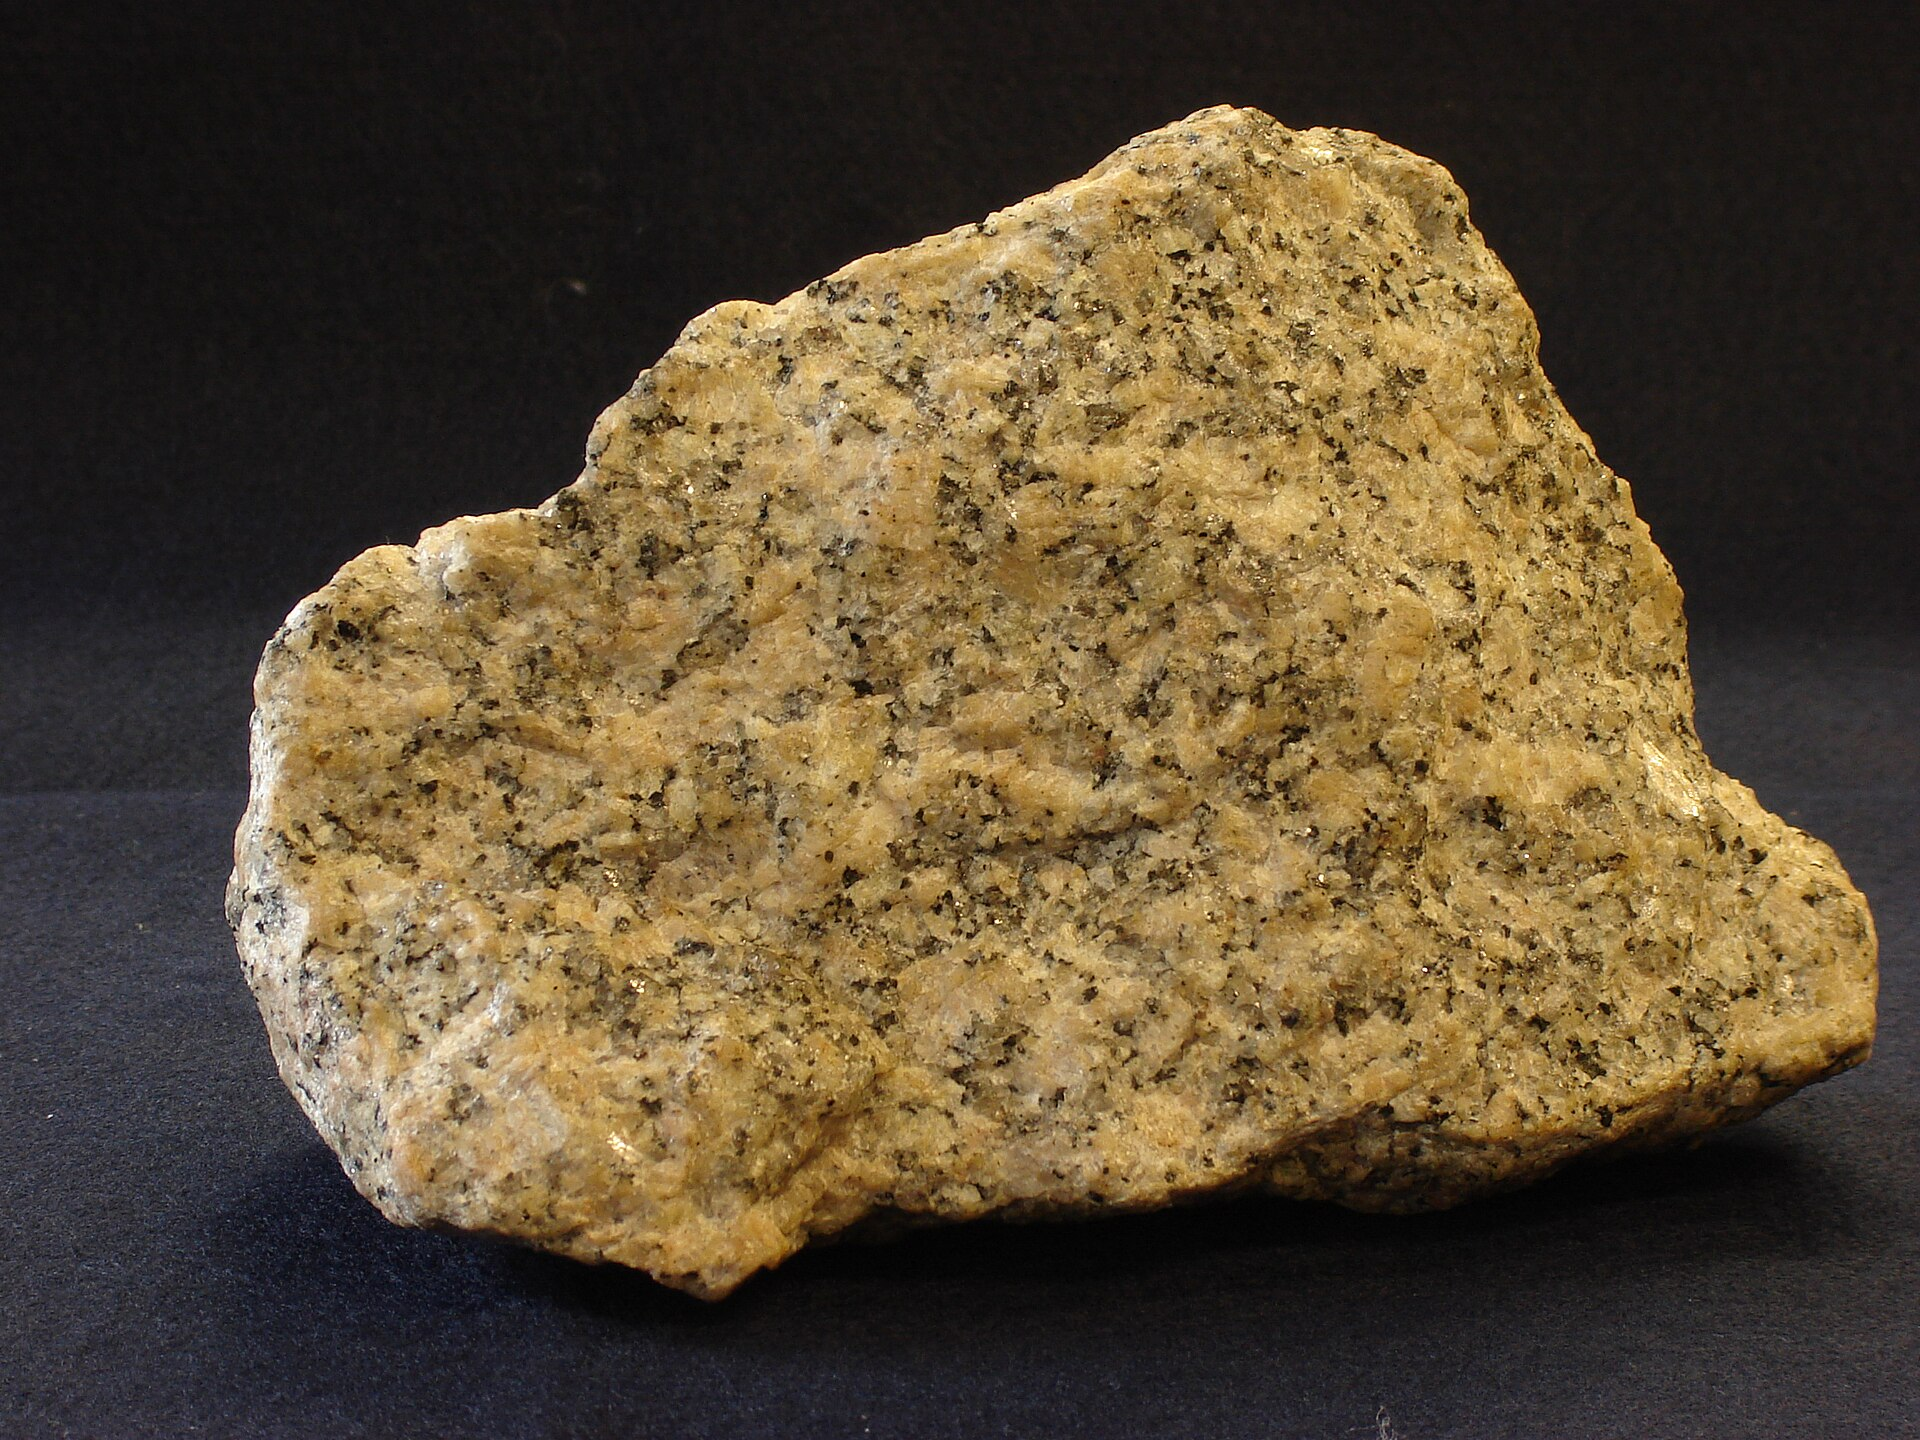
\includegraphics[width=\linewidth,height=4.6cm,keepaspectratio]{images/book1/granite.jpg}

{\small Granite: grains of three or four different minerals can be seen.
A heterogeneous solid. Photo: Eurico Zimbres, CC BY-SA 2.0 br.}
\end{minipage}\hfill
\begin{minipage}[b]{0.48\linewidth}\centering
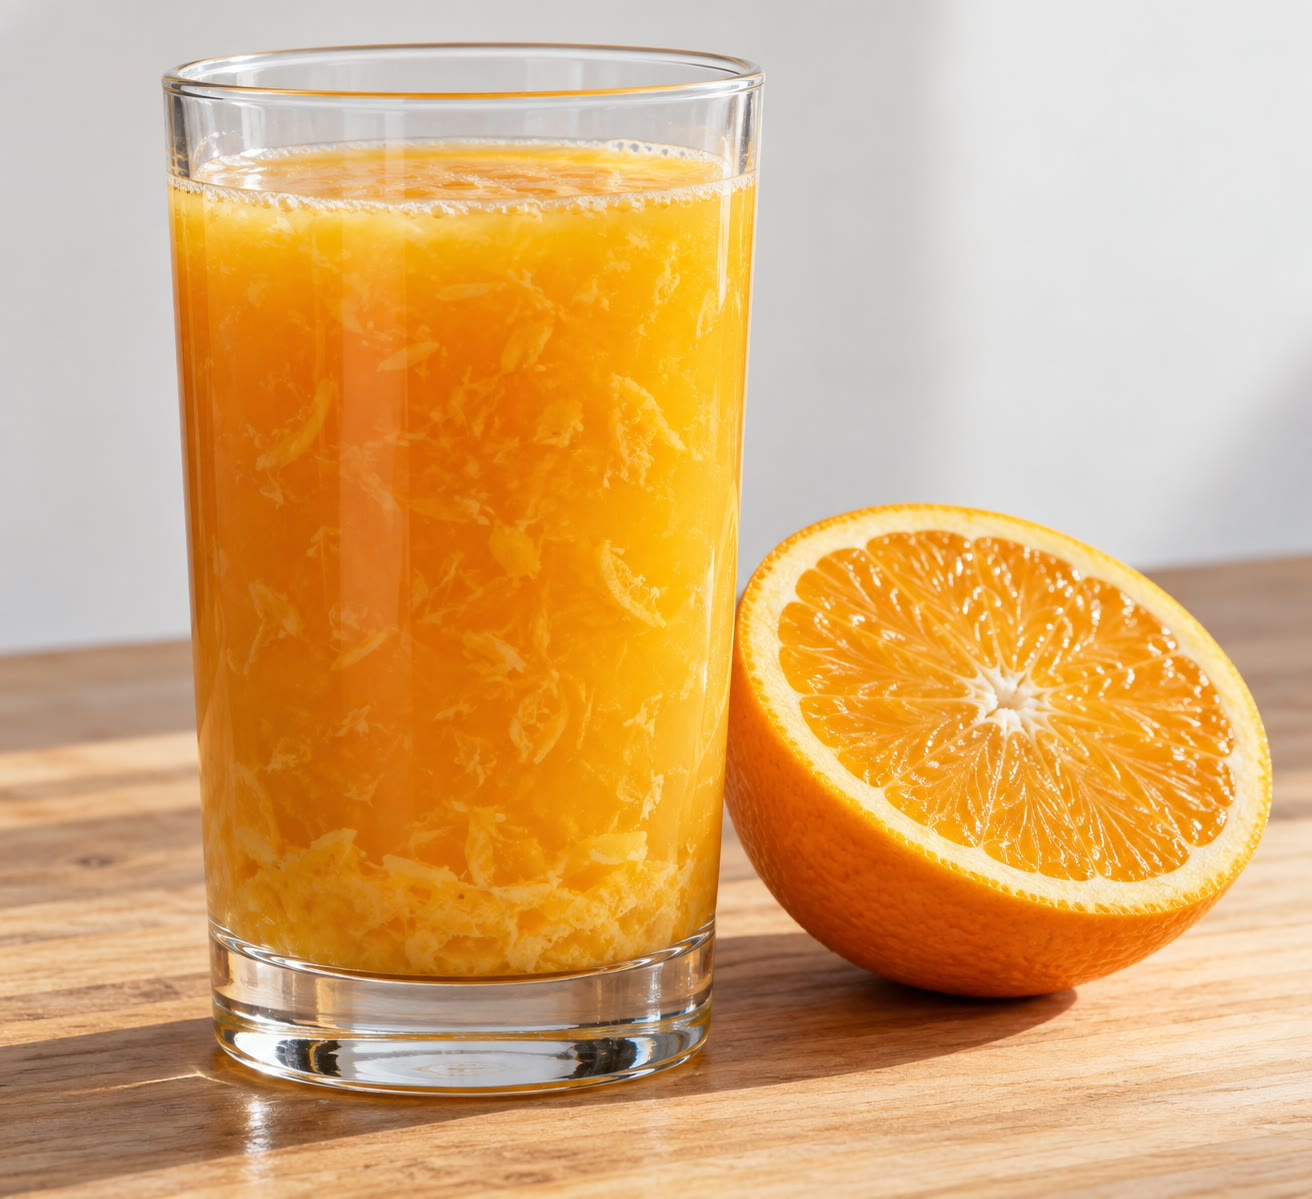
\includegraphics[width=\linewidth,height=4.6cm,keepaspectratio]{images/book1/ai/g6-orange-juice.jpg}

{\small Orange juice with pulp: a \omterm{def:g6:pure-substances-and-mixtures:homogeneous}{heterogeneous mixture}.}
\end{minipage}
\end{omfigure}

\begin{remark}[Homogeneous does not mean pure]\label{rem:g6:pure-substances-and-mixtures:not-pure}
Salty water looks exactly like pure water. Looking is not enough to tell
a \omterm{def:g6:pure-substances-and-mixtures:pure-substance}{pure substance} from a \omterm{def:g6:pure-substances-and-mixtures:homogeneous}{homogeneous mixture}: we must measure something.
\end{remark}

\section{Identifying a pure substance by its constants}

\begin{proposition}[A pure substance has its own constants]\label{prop:g6:pure-substances-and-mixtures:constants}
% ledger: mp:water, bp:water, bp:ethanol, mp:ethanol, rho:water, rho:ethanol, mp:NaCl, mp:Fe, rho:Fe
Each \omterm{def:g6:pure-substances-and-mixtures:pure-substance}{pure substance} melts at its own fixed temperature, boils at its own
fixed temperature (at normal pressure), and has its own mass for a given
volume, its density. These numbers are its constants; the physics book
explains what they measure. For a few \omterm{def:g6:pure-substances-and-mixtures:pure-substance}{pure substances}:
\begin{center}
\small
\begin{tabular}{lccc}
\hline
\omterm{def:g6:pure-substances-and-mixtures:pure-substance}{pure substance} & melts at & boils at & mass of \qty{1}{cm^3} \\
\hline
water & \qty{0}{\celsius} & \qty{100}{\celsius} & about \qty{1.0}{g} \\
ethanol & \qty{-114}{\celsius} & \qty{78}{\celsius} & \qty{0.79}{g} \\
propanone (acetone) & --- & \qty{56}{\celsius} & \qty{0.78}{g} \\
salt (sodium chloride) & \qty{801}{\celsius} & --- & \qty{2.17}{g} \\
iron & \qty{1538}{\celsius} & --- & \qty{7.87}{g} \\
\hline
\end{tabular}
\end{center}
% ledger: bp:acetone, rho:acetone, rho:NaCl
\end{proposition}

\begin{proposition}[A mixture has no fixed boiling temperature]\label{prop:g6:pure-substances-and-mixtures:mixture-boils}
A \omterm{def:g6:pure-substances-and-mixtures:mixture}{mixture} does not boil at one fixed temperature: salty water starts to
boil a little above \qty{100}{\celsius}, and its temperature keeps rising
while it boils, as the water leaves and the salt that stays behind gets
more concentrated.
\end{proposition}

\begin{method}[Is this liquid pure? Which one is it?]\label{met:g6:pure-substances-and-mixtures:identify}
\begin{enumerate}
  \item Heat it, in the laboratory, and read its temperature while it
        boils.
  \item If the temperature stays fixed, the liquid is probably a \omterm{def:g6:pure-substances-and-mixtures:pure-substance}{pure
        substance}: compare that temperature with a table of constants.
  \item If the temperature keeps rising, it is a \omterm{def:g6:pure-substances-and-mixtures:mixture}{mixture}.
  \item Confirm with a second constant, for instance the mass of a known
        volume.
\end{enumerate}
\end{method}

\begin{inthelab}[Boiling salty water]
The teacher heats pure water and salty water side by side, each with a
thermometer in it. The pure water boils at \qty{100}{\celsius} and stays
there as long as it boils. The salty water starts boiling a little above
\qty{100}{\celsius}, and the thermometer creeps upwards minute after
minute.
\end{inthelab}

\section{Water, pure and not}

\begin{example}[Four waters]\label{ex:g6:pure-substances-and-mixtures:waters}
% ledger: sea:salinity
\begin{itemize}
  \item \textbf{Distilled water}, made in a laboratory, is very nearly a
        \omterm{def:g6:pure-substances-and-mixtures:pure-substance}{pure substance}: water and nothing else.
  \item \textbf{Tap water} is a \omterm{def:g6:pure-substances-and-mixtures:homogeneous}{homogeneous mixture}: water with small
        amounts of dissolved substances (a drop dried on a dark plate
        leaves a white ring).
  \item \textbf{Mineral water} is a \omterm{def:g6:pure-substances-and-mixtures:homogeneous}{homogeneous mixture} whose label gives
        the dissolved substances, in milligrams per litre.
  \item \textbf{Sea water} is a \omterm{def:g6:pure-substances-and-mixtures:homogeneous}{homogeneous mixture} holding about
        \qty{35}{g} of salts in each kilogram.
\end{itemize}
\end{example}

\begin{omfigure}
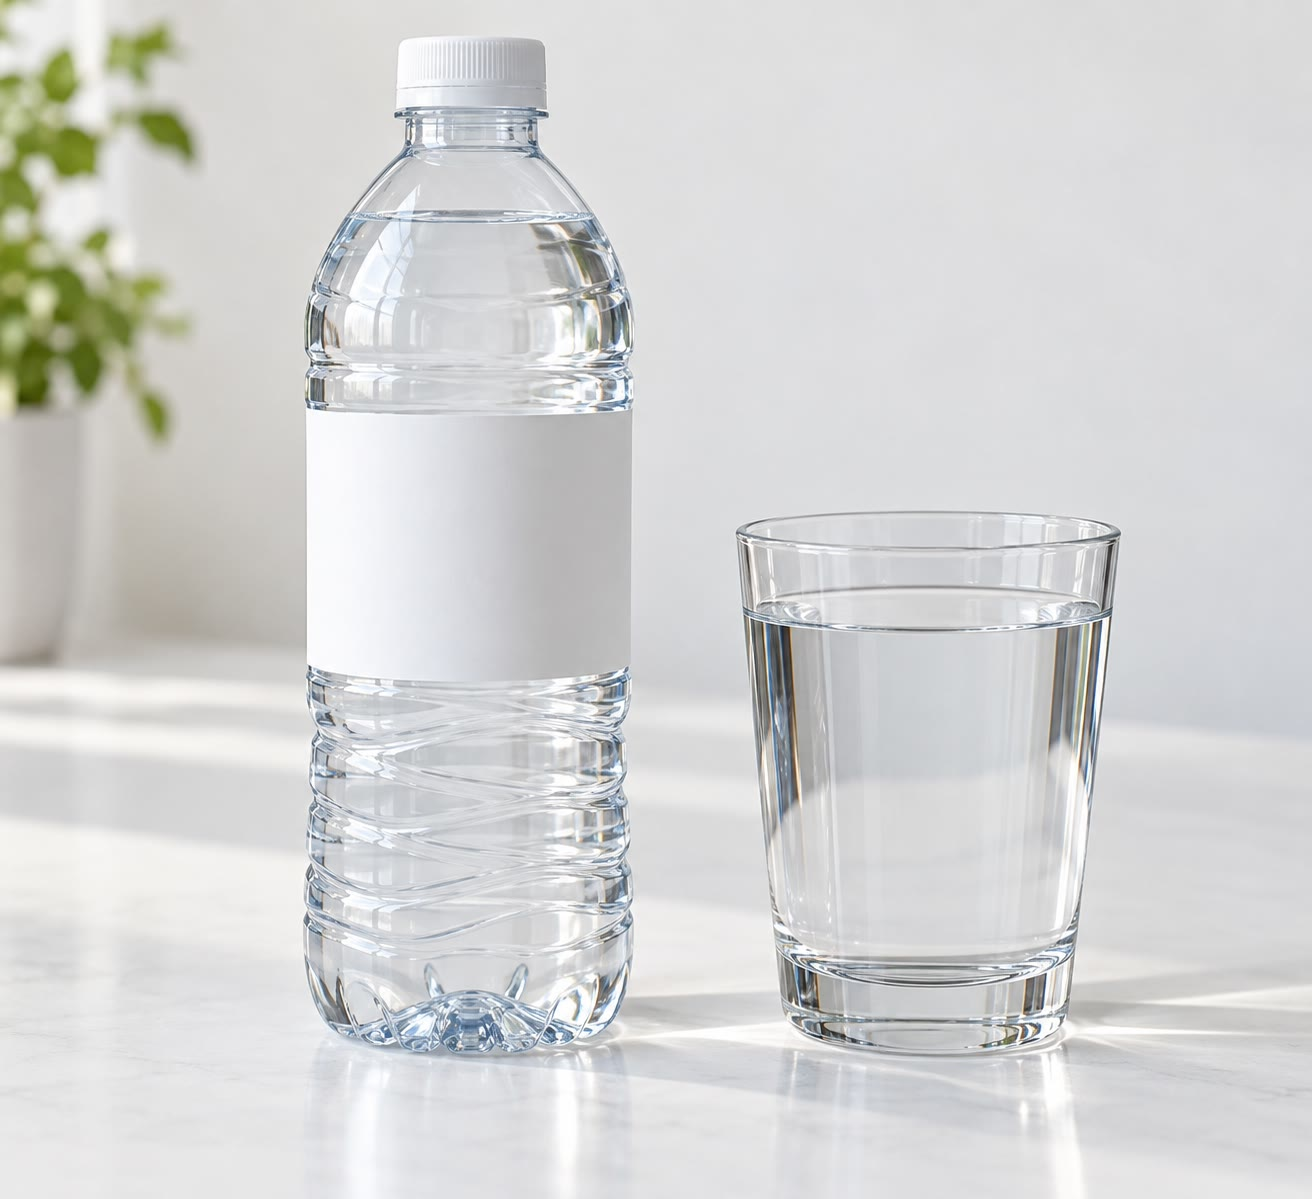
\includegraphics[width=0.5\linewidth]{images/book1/ai/g6-mineral-water.jpg}

{\small A bottle of mineral water: clear and colourless, and still a
\omterm{def:g6:pure-substances-and-mixtures:mixture}{mixture}.}
\end{omfigure}

\begin{example}[Reading a mineral-water label]\label{ex:g6:pure-substances-and-mixtures:label}
A label reads: calcium \qty{78}{mg/L}, magnesium \qty{24}{mg/L},
sodium \qty{5}{mg/L}, hydrogencarbonate \qty{357}{mg/L}, sulfate
\qty{10}{mg/L}, chloride \qty{4}{mg/L}. (These figures are an example.)
In one litre there are $78 + 24 + 5 + 357 + 10 + 4 = 478$\,mg of
dissolved substances, about half a gram: tiny beside the \qty{1000}{g}
of water, but enough to make it a \omterm{def:g6:pure-substances-and-mixtures:mixture}{mixture}.
\end{example}

\section{Exercises}

\begin{exercise}[$\star$]\label{exo:g6:pure-substances-and-mixtures:1}
\omterm{def:g6:pure-substances-and-mixtures:pure-substance}{Pure substance} or \omterm{def:g6:pure-substances-and-mixtures:mixture}{mixture}? Distilled water, \omterm{def:g4:air-a-mixture-of-gases:air}{air}, sea water, a block of
pure iron, milk, a sugar crystal.
\end{exercise}

\begin{exercise}[$\star$]\label{exo:g6:pure-substances-and-mixtures:2}
Homogeneous or heterogeneous? Salty water, granite, oil on water, tap
water, muesli.
\end{exercise}

\begin{exercise}[$\star$]\label{exo:g6:pure-substances-and-mixtures:3}
What is a \omterm{def:g6:pure-substances-and-mixtures:species}{chemical species}? Give three examples.
\end{exercise}

\begin{exercise}[$\star$]\label{exo:g6:pure-substances-and-mixtures:4}
A liquid boils at \qty{78}{\celsius}, and its temperature stays at
\qty{78}{\celsius} while it boils. Use the table of constants to suggest
what it is.
\end{exercise}

\begin{exercise}[$\star$]\label{exo:g6:pure-substances-and-mixtures:5}
Why is ``pure orange juice'' not a \omterm{def:g6:pure-substances-and-mixtures:pure-substance}{pure substance} for a chemist?
\end{exercise}

\begin{exercise}[$\star\star$]\label{exo:g6:pure-substances-and-mixtures:6}
A liquid starts to boil at \qty{100.5}{\celsius} and its temperature
rises while it boils. Is it a \omterm{def:g6:pure-substances-and-mixtures:pure-substance}{pure substance}? What could it be?
\end{exercise}

\begin{exercise}[$\star\star$]\label{exo:g6:pure-substances-and-mixtures:7}
Look at the figure of the four beakers. In which beaker could a filter
separate the parts of the \omterm{def:g6:pure-substances-and-mixtures:mixture}{mixture}? In which beaker could it not?
\end{exercise}

\begin{exercise}[$\star\star$]\label{exo:g6:pure-substances-and-mixtures:8}
A metal cube of volume \qty{10}{cm^3} has a mass of \qty{78.7}{g}. What
is the mass of \qty{1}{cm^3}? Which metal of the table could it be?
\end{exercise}

\begin{exercise}[$\star\star$]\label{exo:g6:pure-substances-and-mixtures:9}
Using the mineral-water label of the example, what percentage of the
dissolved mass is hydrogencarbonate? Round to the nearest whole number.
\end{exercise}

\begin{exercise}[$\star\star$]\label{exo:g6:pure-substances-and-mixtures:10}
Sea water holds about \qty{35}{g} of salts per kilogram. What mass of
salts is there in a \qty{2}{kg} bucket of sea water? What percentage of
the mass of sea water is salt?
\end{exercise}

\begin{exercise}[$\star\star\star$]\label{exo:g6:pure-substances-and-mixtures:11}
Two clear, colourless liquids look identical. Describe two measurements,
made in a laboratory, that would show whether they are the same \omterm{def:g6:pure-substances-and-mixtures:pure-substance}{pure
substance}.
\end{exercise}

\begin{exercise}[$\star\star\star$]\label{exo:g6:pure-substances-and-mixtures:12}
A \omterm{def:g6:pure-substances-and-mixtures:mixture}{mixture} is made of \qty{90}{g} of water and \qty{10}{g} of ethanol.
What percentage of its mass is ethanol? Can it be identified with the
table of constants? Explain.
\end{exercise}

\section{Problem: Three Colourless Liquids}

\begin{problem}[{Weekend problem --- three unlabelled flasks of clear,
colourless liquid, and the measurements that tell them apart}]
\label{pb:g6:pure-substances-and-mixtures:1}
% ledger: bp:water, bp:ethanol, rho:water, rho:ethanol, rho:seawater, sea:salinity
A laboratory assistant finds three flasks, A, B and C, whose labels have
fallen off. All three hold a clear, colourless liquid. The laboratory
uses only three such liquids: distilled water, ethanol and sea water
brought back from a field trip. The assistant makes three kinds of
measurements, in the laboratory.

\medskip
\noindent\textbf{Part I --- Looking.}
\begin{enumerate}
  \item The three liquids look exactly alike. Can the assistant tell, by
        looking, which ones are \omterm{def:g6:pure-substances-and-mixtures:pure-substance}{pure substances}? Explain.
  \item If one of them is a \omterm{def:g6:pure-substances-and-mixtures:mixture}{mixture}, is it homogeneous or heterogeneous?
  \item Which kind of measurement can show that a liquid is a \omterm{def:g6:pure-substances-and-mixtures:pure-substance}{pure
        substance}?
\end{enumerate}

\medskip
\noindent\textbf{Part II --- Measuring.}
Each liquid is heated until it boils. Liquid A boils at
\qty{100}{\celsius} and its temperature stays there. Liquid B boils at
\qty{78}{\celsius} and stays there. Liquid C starts to boil at
\qty{100.6}{\celsius}, and its temperature keeps rising slowly. Then
\qty{50.0}{mL} of each liquid is weighed: A \qty{49.8}{g}, B
\qty{39.5}{g}, C \qty{51.2}{g}.
\begin{enumerate}[resume]
  \item Which liquids are \omterm{def:g6:pure-substances-and-mixtures:pure-substance}{pure substances}? Which is a \omterm{def:g6:pure-substances-and-mixtures:mixture}{mixture}?
  \item Using the table of constants of this chapter, name liquids A and
        B.
  \item Compute the mass of \qty{1}{mL} (that is, \qty{1}{cm^3}) of each
        liquid.
  \item Do these masses agree with your answer to question 5?
  \item Why does the temperature of liquid C keep rising while it boils?
\end{enumerate}

\medskip
\noindent\textbf{Part III --- What is in liquid C?}
\qty{100}{mL} of liquid C are left to dry in a dish. When all the water
has gone, \qty{3.5}{g} of white crystals remain.
\begin{enumerate}[resume]
  \item What does this residue show about liquid C?
  \item Using the mass of \qty{1}{mL} of C found in question 6, find the
        mass of \qty{100}{mL} of C, then the percentage of its mass that
        is salt (to one decimal place).
  \item Sea water holds about \qty{35}{g} of salts in each kilogram. What
        percentage is that? Compare with question 10.
  \item Conclude: how many grams of salt does each litre of liquid C
        hold, and is liquid C the sea water?
\end{enumerate}
\end{problem}
